\documentclass{standalone}
\usepackage{tikz}
\usetikzlibrary{patterns, positioning}

\begin{document}
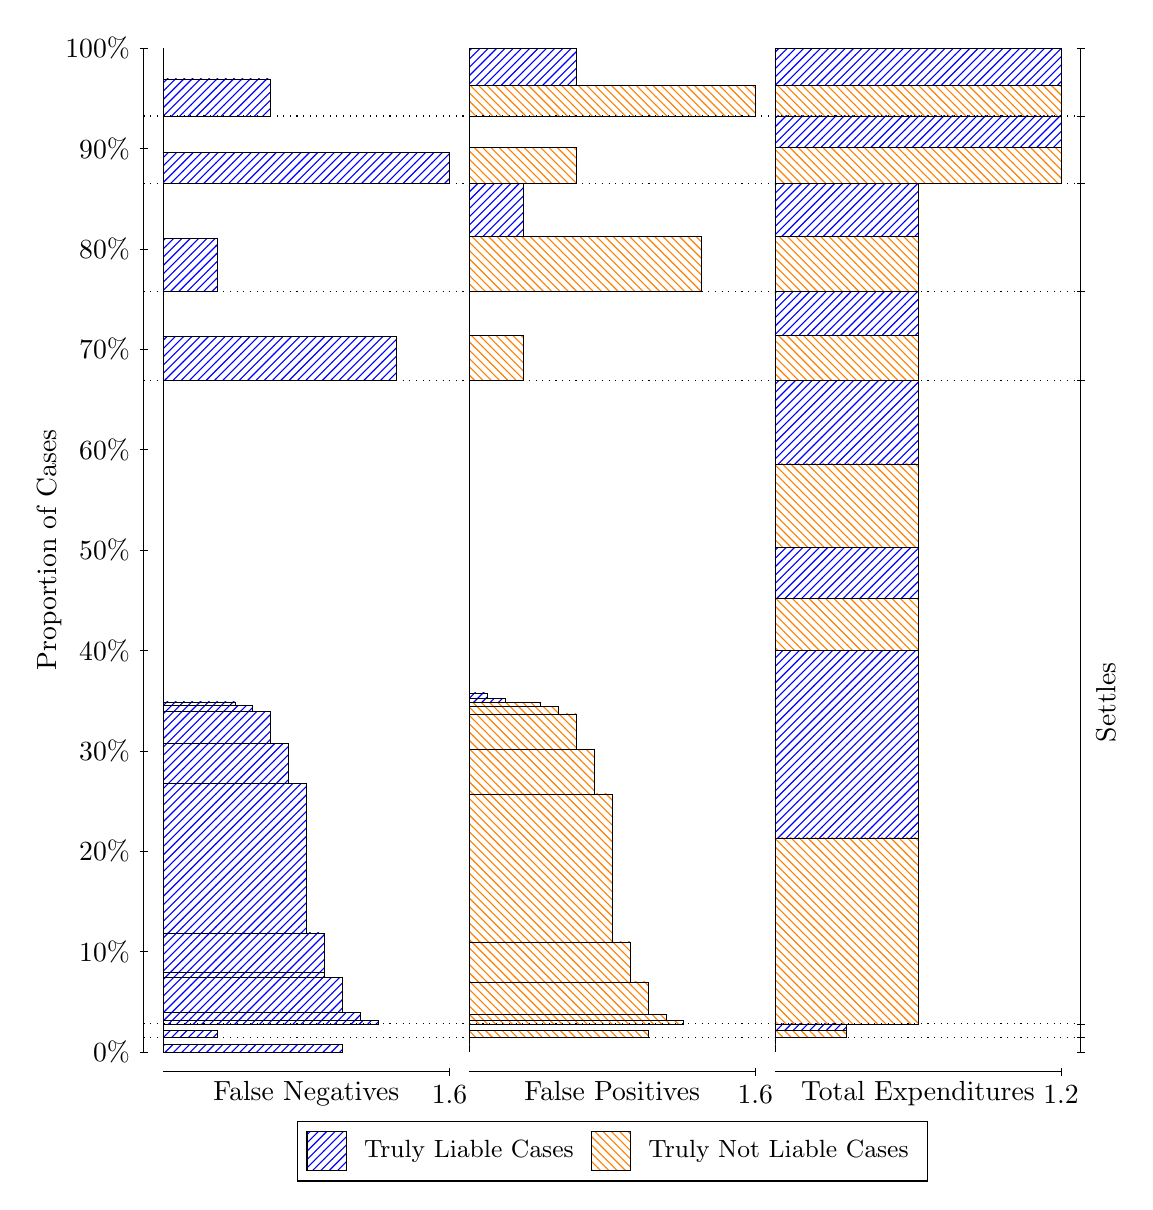
\begin{tikzpicture}
\draw[black, very thin] (1.5,1.75) -- (1.5,14.5);
\node[rotate=90, anchor=center] at (0.3, 8.125) {Proportion of Cases};
\draw[black, very thin] (1.45,1.75) -- (1.55,1.75);
\node[anchor=east] at (1.45, 1.75) {0\%};
\draw[black, very thin] (1.45,3.025) -- (1.55,3.025);
\node[anchor=east] at (1.45, 3.025) {10\%};
\draw[black, very thin] (1.45,4.3) -- (1.55,4.3);
\node[anchor=east] at (1.45, 4.3) {20\%};
\draw[black, very thin] (1.45,5.575) -- (1.55,5.575);
\node[anchor=east] at (1.45, 5.575) {30\%};
\draw[black, very thin] (1.45,6.85) -- (1.55,6.85);
\node[anchor=east] at (1.45, 6.85) {40\%};
\draw[black, very thin] (1.45,8.125) -- (1.55,8.125);
\node[anchor=east] at (1.45, 8.125) {50\%};
\draw[black, very thin] (1.45,9.4) -- (1.55,9.4);
\node[anchor=east] at (1.45, 9.4) {60\%};
\draw[black, very thin] (1.45,10.675) -- (1.55,10.675);
\node[anchor=east] at (1.45, 10.675) {70\%};
\draw[black, very thin] (1.45,11.95) -- (1.55,11.95);
\node[anchor=east] at (1.45, 11.95) {80\%};
\draw[black, very thin] (1.45,13.225) -- (1.55,13.225);
\node[anchor=east] at (1.45, 13.225) {90\%};
\draw[black, very thin] (1.45,14.5) -- (1.55,14.5);
\node[anchor=east] at (1.45, 14.5) {100\%};

\draw[black, very thin] (13.4,1.75) -- (13.4,14.5);
\draw[black, very thin] (13.35,1.75) -- (13.45,1.75);
\node[anchor=west] at (13.35, 1.75) {};
\draw[black, very thin] (13.35,1.9371) -- (13.45,1.9371);
\node[anchor=west] at (13.35, 1.9371) {};
\draw[black, very thin] (13.35,2.1067) -- (13.45,2.1067);
\node[anchor=west] at (13.35, 2.1067) {};
\draw[black, very thin] (13.35,10.278) -- (13.45,10.278);
\node[anchor=west] at (13.35, 10.278) {};
\draw[black, very thin] (13.35,11.408) -- (13.45,11.408);
\node[anchor=west] at (13.35, 11.408) {};
\draw[black, very thin] (13.35,12.777) -- (13.45,12.777);
\node[anchor=west] at (13.35, 12.777) {};
\draw[black, very thin] (13.35,13.637) -- (13.45,13.637);
\node[anchor=west] at (13.35, 13.637) {};
\draw[black, very thin] (13.35,14.5) -- (13.45,14.5);
\node[anchor=west] at (13.35, 14.5) {};

\draw[black, very thin, pattern color=blue, pattern=north east lines] (1.75,1.75) rectangle (4.0208,1.8428);
\draw[black, very thin, pattern color=orange, pattern=north west lines] (1.75,1.8428) rectangle (1.75,1.9371);
\draw[black, very thin, pattern color=blue, pattern=north east lines] (1.75,1.9371) rectangle (2.4312,2.0219);
\draw[black, very thin, pattern color=orange, pattern=north west lines] (1.75,2.0219) rectangle (1.75,2.1067);
\draw[black, very thin, pattern color=blue, pattern=north east lines] (1.75,2.1067) rectangle (4.475,2.1549);
\draw[black, very thin, pattern color=blue, pattern=north east lines] (1.75,2.1549) rectangle (4.2479,2.2488);
\draw[black, very thin, pattern color=blue, pattern=north east lines] (1.75,2.2488) rectangle (4.0208,2.694);
\draw[black, very thin, pattern color=blue, pattern=north east lines] (1.75,2.694) rectangle (3.7937,2.7594);
\draw[black, very thin, pattern color=blue, pattern=north east lines] (1.75,2.7594) rectangle (3.7937,3.2627);
\draw[black, very thin, pattern color=blue, pattern=north east lines] (1.75,3.2627) rectangle (3.5667,5.159);
\draw[black, very thin, pattern color=blue, pattern=north east lines] (1.75,5.159) rectangle (3.3396,5.6658);
\draw[black, very thin, pattern color=blue, pattern=north east lines] (1.75,5.6658) rectangle (3.1125,6.0734);
\draw[black, very thin, pattern color=blue, pattern=north east lines] (1.75,6.0734) rectangle (2.8854,6.1476);
\draw[black, very thin, pattern color=blue, pattern=north east lines] (1.75,6.1476) rectangle (2.6583,6.1952);
\draw[black, very thin, pattern color=orange, pattern=north west lines] (1.75,6.1952) rectangle (1.75,10.278);
\draw[black, very thin, pattern color=blue, pattern=north east lines] (1.75,10.278) rectangle (4.7021,10.84);
\draw[black, very thin, pattern color=orange, pattern=north west lines] (1.75,10.84) rectangle (1.75,11.408);
\draw[black, very thin, pattern color=blue, pattern=north east lines] (1.75,11.408) rectangle (2.4312,12.082);
\draw[black, very thin, pattern color=orange, pattern=north west lines] (1.75,12.082) rectangle (1.75,12.777);
\draw[black, very thin, pattern color=blue, pattern=north east lines] (1.75,12.777) rectangle (5.3833,13.177);
\draw[black, very thin, pattern color=orange, pattern=north west lines] (1.75,13.177) rectangle (1.75,13.637);
\draw[black, very thin, pattern color=blue, pattern=north east lines] (1.75,13.637) rectangle (3.1125,14.109);
\draw[black, very thin, pattern color=orange, pattern=north west lines] (1.75,14.109) rectangle (1.75,14.5);
\draw[black, very thin, pattern color=orange, pattern=north west lines] (5.6333,1.75) rectangle (5.6333,1.8443);
\draw[black, very thin, pattern color=blue, pattern=north east lines] (5.6333,1.8443) rectangle (5.6333,1.9371);
\draw[black, very thin, pattern color=orange, pattern=north west lines] (5.6333,1.9371) rectangle (7.9042,2.0219);
\draw[black, very thin, pattern color=blue, pattern=north east lines] (5.6333,2.0219) rectangle (5.6333,2.1067);
\draw[black, very thin, pattern color=orange, pattern=north west lines] (5.6333,2.1067) rectangle (8.3583,2.1555);
\draw[black, very thin, pattern color=orange, pattern=north west lines] (5.6333,2.1555) rectangle (8.1313,2.2308);
\draw[black, very thin, pattern color=orange, pattern=north west lines] (5.6333,2.2308) rectangle (7.9042,2.6399);
\draw[black, very thin, pattern color=orange, pattern=north west lines] (5.6333,2.6399) rectangle (7.6771,3.1473);
\draw[black, very thin, pattern color=orange, pattern=north west lines] (5.6333,3.1473) rectangle (7.45,5.0266);
\draw[black, very thin, pattern color=orange, pattern=north west lines] (5.6333,5.0266) rectangle (7.2229,5.5959);
\draw[black, very thin, pattern color=orange, pattern=north west lines] (5.6333,5.5959) rectangle (6.9958,6.0445);
\draw[black, very thin, pattern color=orange, pattern=north west lines] (5.6333,6.0445) rectangle (6.7687,6.1398);
\draw[black, very thin, pattern color=orange, pattern=north west lines] (5.6333,6.1398) rectangle (6.5417,6.1891);
\draw[black, very thin, pattern color=blue, pattern=north east lines] (5.6333,6.1891) rectangle (6.0875,6.2367);
\draw[black, very thin, pattern color=blue, pattern=north east lines] (5.6333,6.2367) rectangle (5.8604,6.3109);
\draw[black, very thin, pattern color=blue, pattern=north east lines] (5.6333,6.3109) rectangle (5.6333,10.278);
\draw[black, very thin, pattern color=orange, pattern=north west lines] (5.6333,10.278) rectangle (6.3146,10.847);
\draw[black, very thin, pattern color=blue, pattern=north east lines] (5.6333,10.847) rectangle (5.6333,11.408);
\draw[black, very thin, pattern color=orange, pattern=north west lines] (5.6333,11.408) rectangle (8.5854,12.103);
\draw[black, very thin, pattern color=blue, pattern=north east lines] (5.6333,12.103) rectangle (6.3146,12.777);
\draw[black, very thin, pattern color=orange, pattern=north west lines] (5.6333,12.777) rectangle (6.9958,13.236);
\draw[black, very thin, pattern color=blue, pattern=north east lines] (5.6333,13.236) rectangle (5.6333,13.637);
\draw[black, very thin, pattern color=orange, pattern=north west lines] (5.6333,13.637) rectangle (9.2667,14.028);
\draw[black, very thin, pattern color=blue, pattern=north east lines] (5.6333,14.028) rectangle (6.9958,14.5);
\draw[black, very thin, pattern color=orange, pattern=north west lines] (9.5167,1.75) rectangle (9.5167,1.8443);
\draw[black, very thin, pattern color=blue, pattern=north east lines] (9.5167,1.8443) rectangle (9.5167,1.9371);
\draw[black, very thin, pattern color=orange, pattern=north west lines] (9.5167,1.9371) rectangle (10.425,2.0219);
\draw[black, very thin, pattern color=blue, pattern=north east lines] (9.5167,2.0219) rectangle (10.425,2.1067);
\draw[black, very thin, pattern color=orange, pattern=north west lines] (9.5167,2.1067) rectangle (11.333,4.4703);
\draw[black, very thin, pattern color=blue, pattern=north east lines] (9.5167,4.4703) rectangle (11.333,6.8485);
\draw[black, very thin, pattern color=orange, pattern=north west lines] (9.5167,6.8485) rectangle (11.333,7.5086);
\draw[black, very thin, pattern color=blue, pattern=north east lines] (9.5167,7.5086) rectangle (11.333,8.1613);
\draw[black, very thin, pattern color=orange, pattern=north west lines] (9.5167,8.1613) rectangle (11.333,9.22);
\draw[black, very thin, pattern color=blue, pattern=north east lines] (9.5167,9.22) rectangle (11.333,10.278);
\draw[black, very thin, pattern color=orange, pattern=north west lines] (9.5167,10.278) rectangle (11.333,10.847);
\draw[black, very thin, pattern color=blue, pattern=north east lines] (9.5167,10.847) rectangle (11.333,11.408);
\draw[black, very thin, pattern color=orange, pattern=north west lines] (9.5167,11.408) rectangle (11.333,12.103);
\draw[black, very thin, pattern color=blue, pattern=north east lines] (9.5167,12.103) rectangle (11.333,12.777);
\draw[black, very thin, pattern color=orange, pattern=north west lines] (9.5167,12.777) rectangle (13.15,13.236);
\draw[black, very thin, pattern color=blue, pattern=north east lines] (9.5167,13.236) rectangle (13.15,13.637);
\draw[black, very thin, pattern color=orange, pattern=north west lines] (9.5167,13.637) rectangle (13.15,14.028);
\draw[black, very thin, pattern color=blue, pattern=north east lines] (9.5167,14.028) rectangle (13.15,14.5);
\draw[black, dotted] (1.5,1.9371) -- (13.4,1.9371);
\draw[black, dotted] (1.5,2.1067) -- (13.4,2.1067);
\draw[black, dotted] (1.5,10.278) -- (13.4,10.278);
\draw[black, dotted] (1.5,11.408) -- (13.4,11.408);
\draw[black, dotted] (1.5,12.777) -- (13.4,12.777);
\draw[black, dotted] (1.5,13.637) -- (13.4,13.637);
\draw[black, very thin] (1.75,1.5) -- (5.3833,1.5);
\node[anchor=north] at (3.5667, 1.5) {False Negatives};
\draw[black, very thin] (5.3833,1.45) -- (5.3833,1.55);
\node[anchor=north] at (5.3833, 1.45) {1.6};

\draw[black, very thin] (5.6333,1.5) -- (9.2667,1.5);
\node[anchor=north] at (7.45, 1.5) {False Positives};
\draw[black, very thin] (9.2667,1.45) -- (9.2667,1.55);
\node[anchor=north] at (9.2667, 1.45) {1.6};

\draw[black, very thin] (9.5167,1.5) -- (13.15,1.5);
\node[anchor=north] at (11.333, 1.5) {Total Expenditures};
\draw[black, very thin] (13.15,1.45) -- (13.15,1.55);
\node[anchor=north] at (13.15, 1.45) {1.2};



\node[black, centered, rotate=90] at (13.72, 6.1922) {Settles};





\draw (7.449999999999999,1.5) node[draw=none] (baseCoordinate) {};
\begin{scope}[align=center]
        \matrix[scale=0.5, draw=black, below=0.5cm of baseCoordinate, nodes={draw}, column sep=0.1cm]{
            \node[rectangle, draw, minimum width=0.5cm, minimum height=0.5cm, pattern=north east lines, pattern color=blue] {}; &
            \node[draw=none, font=\small] (B) {Truly Liable Cases}; &
            \node[rectangle, draw, minimum width=0.5cm, minimum height=0.5cm, pattern=north west lines, pattern color=orange] {}; &
            \node[draw=none, font=\small] (B) {Truly Not Liable Cases}; \\
            };
\end{scope}

\end{tikzpicture}
\end{document}